\documentclass[a4paper]{article}
\title{Sweave Example 1} 
\author{Steve}
\usepackage{Sweave} 
\begin{document}
\Sconcordance{concordance:examp15.tex:examp15.Rnw:%
1 8 1 1 2 4 0 1 2 14 1 1 2 5 0 1 2}

\maketitle
\section{Section 1}
This is section one. Blah, blah, etc.
\begin{Schunk}
\begin{Sinput}
> my.lm = lm(mpg~wt,data=mtcars)
\end{Sinput}
\end{Schunk}

\begin{table}[ht]
\centering
\begin{tabular}{rrrrr}
  \hline
 & Estimate & Std. Error & t value & Pr($>$$|$t$|$) \\ 
  \hline
(Intercept) & 37.2851 & 1.8776 & 19.86 & 0.0000 \\ 
  wt & -5.3445 & 0.5591 & -9.56 & 0.0000 \\ 
   \hline
\end{tabular}
\end{table} 

\section{Section 2}
Here we do some regression
\begin{Schunk}
\begin{Sinput}
> plot(my.lm)
\end{Sinput}
\end{Schunk}
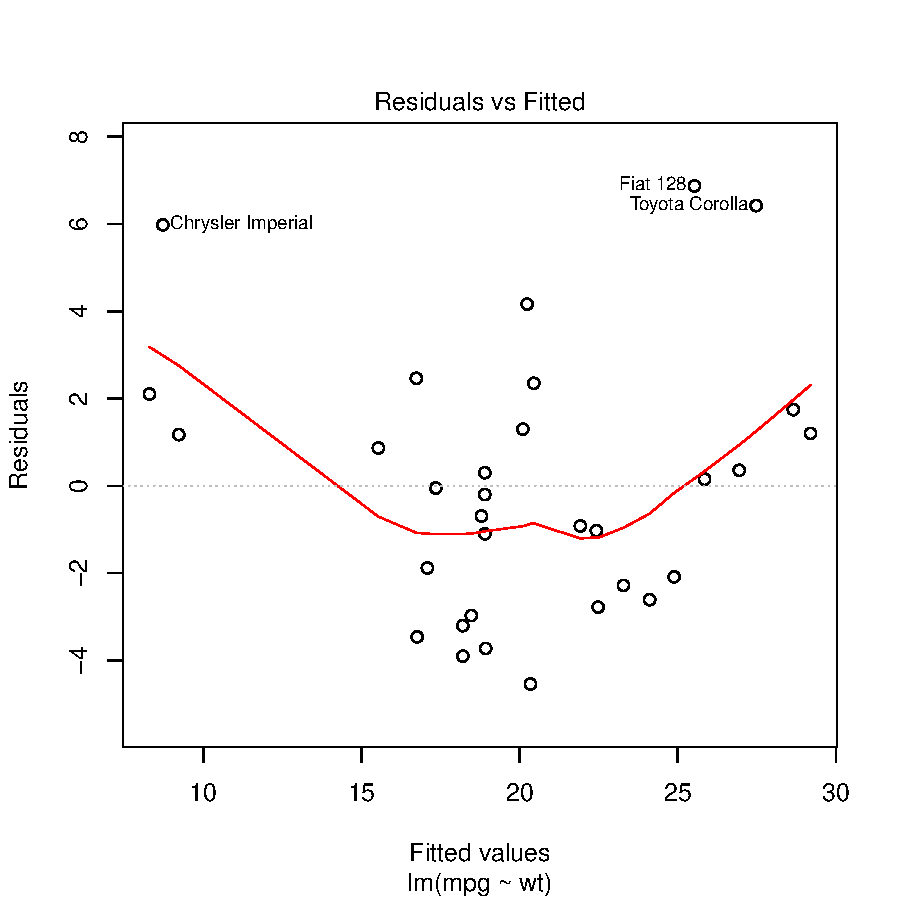
\includegraphics{examp15-002}
\end{document}
